% Set up the document
\documentclass{article}

% Page size
\usepackage[
    letterpaper,]{geometry}

% Lines between paragraphs
\setlength{\parskip}{\baselineskip}
\setlength{\parindent}{0pt}

% Math
\usepackage{mathtools}
\usepackage{amssymb}
\usepackage{amsthm}
\usepackage{commath}

% Operators
\DeclareMathOperator{\tr}{tr}

% Number sets
\newcommand{\C}{\mathbb{C}}
\newcommand{\N}{\mathbb{N}}
\newcommand{\Q}{\mathbb{Q}}
\newcommand{\R}{\mathbb{R}}
\newcommand{\Z}{\mathbb{Z}}

% Links
\usepackage{hyperref}

% Page numbers at top right
\usepackage{fancyhdr}
\pagestyle{fancy}
\fancyhf{}
\fancyhead[R]{\thepage}
\renewcommand\headrulewidth{0pt}

% Graphics
\usepackage{float}
\usepackage{graphicx}
\graphicspath{ {./img/} }

\begin{document}

\textbf{MATH 461 assignment 3} \\
\textbf{Matt Wiens \#301294492} \\
\textbf{2020-06-26}

3.9.4. In this exercise, you will be considering three simple models of
a fishery. Let $N(t)$ be the population of fish at time $t$. In the
absence of fishing, the population is assumed to grow logistically,
that is,
%
\begin{equation*}
    \dot N = r N \del{1 - \frac{N}{K}}
    ,
\end{equation*}
%
where $r > 0$ is the intrinsic growth of the population, and $K >0$ is
the carrying capacity for the fish population. The effects of fishing
are modeled with an additional term in the equation for $N$. The three
models are as follows:
%
\begin{align*}
    \text{\textbf{Model 1:}} \ \dot N &= r N \del{1 - \frac{N}{K}} - H_1; \\
    \text{\textbf{Model 2:}} \ \dot N &= r N \del{1 - \frac{N}{K}} - H_2 N; \\
    \text{\textbf{Model 3:}} \ \dot N &= r N \del{1 - \frac{N}{K}} - H_3 \frac{A}{A + N},
\end{align*}
%
where $H_1$, $H_2$, $H_3$, and $A$ are positive constants.

(a) For each model, give a biological interpretation of the fishing
term. How do they differ? What is the meaning of the constants $H_1$,
$H_2$, $H_3$, and $A$?

\textit{Solution.}
For all three models, the $H_1$, $H_2 N$, and $H_3 \frac{A}{A + N}$
terms are rates which determines how many fish are removed from the
population by the fishery per unit time.

The first rate, $H_1$, is constant, in contrast to the other two models,
and does not depend on the population size $N$. If time was measured in
units of days for example, then, biologically speaking, $H_1$ would tell
us how many fish to remove from the population each day.

In the second rate, $H_2 N$, the $H_2$ term tells the proportion of the
population $N$ to remove per unit time. The rate $H_2 N$ is clearly
directly proportional to the population---higher population, remove more
fish; lower population, remove fewer fish.

The third rate, $H_3 \frac{A}{A + N}$, is more complicated. As in the
first model, the $H_3$ term tells us how many fish to remove per unit
time; however this is scaled by a population-dependent fractional term.
In order for the fractional term $\frac{A}{A + N}$ to make sense, $A$
must be in units of fish (it could represent some ``canonical''
population size, for example). Interpreting this term as a scaling
factor for the $H_3$ term, for any given $A$, higher populations lead to
fewer fish being removed and lower populations lead to more fish being
removed; this is in some sense opposite to how the second model's
harvesting works. The smaller the $A$ term, the more strongly the
population size $N$ affects the scaling term.


\vspace{5mm}

(b) Critique model 1. Why is it not biologically realistic?

\textit{Solution.}
The biggest problem with model 1 is that, because the harvesting is
constant, the population can theoretically take on negative values. It
also makes much more sense to base the harvesting rate on the population
size, as is done in the other models, to optimize harvesting yields
while keeping the population stable.

\vspace{5mm}

(c) Which of Models 2 or 3 do you think is best and why?

\textit{Solution.}
I honestly don't understand the context in which model 3 makes sense.
Model 2, however, makes a lot of sense to me. The more fish you have,
the more you can afford to harvest while maintaining a stable
population, and, similarly, the fewer fish you have, the less you can
afford to harvest while maintaining stability. The logic for model 3
is opposite to this.

\newpage

3.9.5. Levins suggested modeling not the number of individuals but the
fraction of patches that a population occupies. He suggested the
following equation:
%
\begin{equation*}
    P^\prime = c P (h - P) - \mu P
    ,
\end{equation*}
%
where $P(t)$ denotes the fraction of occupied patches. The number $h$
denotes the fraction of patches that is actually habitable for the
population and hence $h - P$ is the number of empty but habitable
patches. Note that $0 \leq P \leq h \leq 1$. The population colonizes
empty patches with rate $c$. Occupied patches become empty with rate
$\mu$.

(a) Find the steady states of the system.

\textit{Solution.}
To find the steady states, we set $P^\prime = 0$, so
%
\begin{equation*}
    c P (h - P) - \mu P = 0
    .
\end{equation*}
%
Clearly $P = 0$ is a solution. For $P \neq 0$, we have
%
\begin{align*}
    &c P (h - P) - \mu P = 0 \\
    &\iff c (h - P) - \mu = 0 \\
    &\iff P = h - \frac{\mu}{c}
    .
\end{align*}
%
Hence the steady states are given by $P_0 = 0$, $P_1 = h - \mu / c$.

\vspace{5mm}

(b) Assume that $h$ can be varied (e.g., construction takes up habitable
patches). Draw the bifurcation diagram with $h$ as the parameter. Do all
the habitable patches have to be destroyed before the population dies
out?

\textit{Solution.}
Setting $f(P, h) = c P (h - P) - \mu P$, the solution to
%
\begin{align*}
    f(\bar{P}, \bar{h}) &= 0, \\
    \dpd{f}{P}(\bar{P}, \bar{h}) &= 0,
\end{align*}
%
is $\bar{P} = 0$, $\bar{h} = \mu / c$ (I used Maple for this).
This tells us the bifurcation point and corresponding bifurcation value.
Hence we can see right away that not all habitable patches need to be destroyed
before the population dies out.

Now we need to assess the stability of the steady state when $h > \mu /
c$. Here we'll take $P = h - \mu / c + \epsilon$ and substitute it into
our initial differential equation:
%
\begin{align*}
    P^\prime
        &=
        c \del{h - \frac{\mu}{c}+ \epsilon}
        \del{h - \del{h - \frac{\mu}{c} + \epsilon}}
        - \mu \del{h - \frac{\mu}{c} + \epsilon} \\
        &= - \epsilon ((\epsilon + h) c - \mu)
\end{align*}
%
Hence taking the limit of $\epsilon \to 0$ we see that solutions are
stable provided that $h c > \mu$. This is because if we increase the
population size by a small amount $\epsilon$, then if the condition
holds, $P^\prime < 0$. Similarly if we decrease the population by a
small amount then the derivative becomes negative. The states are
unstable if $hc < \mu$, by similar logic. If $hc = \mu$ then
the derivative reduces to $P^\prime = - c \epsilon^2$ so this is
also not stable.

The bifurcation diagram is shown in Figure~\ref{fig:395}.

\begin{figure}[!ht]
    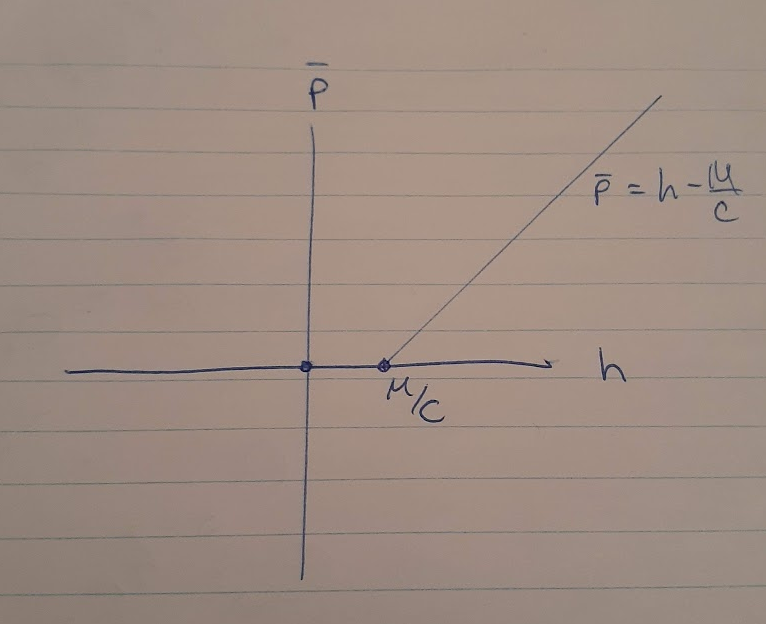
\includegraphics[width=3.7in]{q395}
    \centering
    \caption{Bifurcation diagram}
    \label{fig:395}
\end{figure}

\newpage

3.9.6. Consider a gene that is activated by the presence of a
biochemical substance $S$. Let $g(t)$ denote the concentration of the
gene product at time $t$, and assume that the concentration of $S$,
denoted by $s_0$, is fixed. A model describing the dynamics of $g$
is as follows:
%
\begin{equation}
    \dod{g}{t} = k_1 s_0 - k_2 g + \frac{k_3 g^2}{k_4^2 + g^2}
    \label{eq:396-1}
    ,
\end{equation}
%
where the $k$'s are positive constants.

(b) Show that~\eqref{eq:396-1} can be put in the dimensionless form
%
\begin{equation*}
    \dod{x}{\tau} = s - r x + \frac{x^2}{1 + x^2}
    ,
\end{equation*}
%
where $r > 0$ and $s \geq 0$ are dimensionless groups. What are $r$ and
$s$ in terms of the original model parameters?

\textit{Solution.}
First, note that the constants $k_1, k_2$ have units of inverse time,
$k_3$ has units of concentration over time, while the constant $k_4$ has
units of concentration. As a first step, we can write
%
\begin{align*}
    \tau &= \frac{k_3}{k_4} t, \\
    x(\tau) &= \frac{1}{k_4} g\del{\frac{k_4 \tau}{k_3}}
    ,
\end{align*}
%
and using the chain rule we have
%
\begin{equation*}
    \dod{x}{\tau} = \frac{1}{k_4} \dod{t}{\tau} \dod{g}{t} = \frac{1}{k_3} \dod{g}{t}
    .
\end{equation*}

Hence we can write~\eqref{eq:396-1} as
%
\begin{equation*}
    k_3 \dod{x}{\tau} = k_1 s_0 - k_2 k_4 x + k_3 \frac{x^2}{1 + x^2}
    .
\end{equation*}
%
Dividing through by $k_3$ we have
%
\begin{equation*}
    \dod{x}{\tau} = \frac{k_1}{k_3} s_0 - \frac{k_2 k_4}{k_3} x + \frac{x^2}{1 + x^2}
    .
\end{equation*}
%
Now, for the dimensionless groups, we clearly have
%
\begin{align*}
    s &= \frac{k_1}{k_3} s_0, \\
    r &= \frac{k_2 k_4}{k_3}
    .
\end{align*}

\newpage

3.9.7. We study $2 \times 2$ systems of linear ODEs:
%
\begin{equation*}
    y^\prime = A y, \quad
    y =
    \begin{pmatrix}
        y_1 \\
        y_2
    \end{pmatrix}, \quad
    A =
    \begin{pmatrix}
        a & b \\
        c & d
    \end{pmatrix}
    .
\end{equation*}
%
Classify the origin $\begin{pmatrix}0 \\ 0\end{pmatrix}$ as either
stable/unstable spiral, node, or saddle, and plot (or sketch) the
phase portrait for each of the following cases:
%
\begin{equation*}
    A =
    \begin{pmatrix}
        1 & 1 \\
        3 & -1
    \end{pmatrix}
    ,
    \begin{pmatrix}
        2 & 1 \\
        2 & 3
    \end{pmatrix}
    ,
    \begin{pmatrix}
        -1 & -2 \\
        2 & -1
    \end{pmatrix}
    .
\end{equation*}

\textit{Solution.}
For each of these matrices we find the determinant and trace. We then
use Theorem 3.3 from the course textbook to determine stability. Having
done that, we will plot the phase portrait.

We first consider
%
\begin{equation*}
    A_1 =
    \begin{pmatrix}
        1 & 1 \\
        3 & -1
    \end{pmatrix}
    ,
\end{equation*}
%
which has
%
\begin{align*}
    \det A_1 &= 1 \cdot (-1) - 1 \cdot 3 = -4, \\
    \tr A_1 &= 1 + (-1) = 0
    .
\end{align*}
%
Since $\det A_1 < 0$, according to Theorem 3.3, the center is not
stable. The origin is a saddle, as shown in Figure~\ref{fig:397-a}.

\begin{figure}[!ht]
    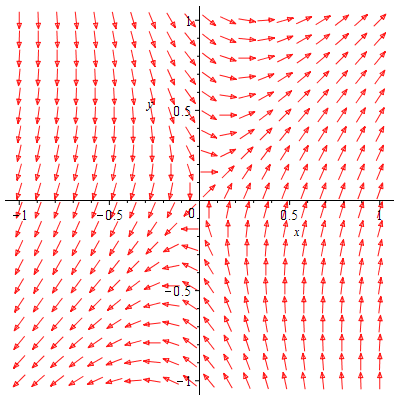
\includegraphics[width=3.7in]{q397a}
    \centering
    \caption{Phase portrait of the first system}
    \label{fig:397-a}
\end{figure}

Next we have
%
\begin{equation*}
    A_2 =
    \begin{pmatrix}
        2 & 1 \\
        2 & 3
    \end{pmatrix}
    ,
\end{equation*}
%
with
%
\begin{align*}
    \det A_2 &= 2 \cdot 3 - 1 \cdot 2 = 4, \\
    \tr A_2 &= 2 + 3 = 5
    .
\end{align*}
%
Theorem 3.3 again tells us the center is not stable, since
$\tr A_2 > 0$. The origin is an unstable node, as shown in
Figure~\ref{fig:397-b}.

\begin{figure}[!ht]
    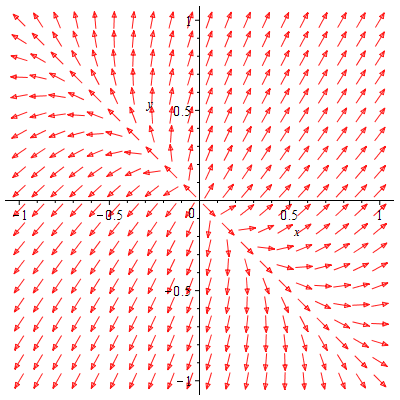
\includegraphics[width=3.7in]{q397b}
    \centering
    \caption{Phase portrait of the second system}
    \label{fig:397-b}
\end{figure}

Finally we have
%
\begin{equation*}
    A_3 =
    \begin{pmatrix}
        -1 & -2 \\
        2 & -1
    \end{pmatrix}
    ,
\end{equation*}
%
with
%
\begin{align*}
    \det A_3 &= (-1) \cdot (-1) - (-2) \cdot 2 = 5, \\
    \tr A_3 &= (-1) + (-1) = -2
    .
\end{align*}
%
Theorem 3.3 tells us the center is asymptotically stable, since $\det A_3
> 0$ and $\tr A_3 < 0$. The origin is a stable spiral, as shown in
Figure~\ref{fig:397-c}.

\begin{figure}[!ht]
    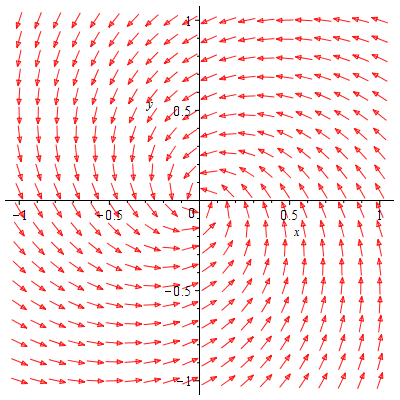
\includegraphics[width=3.7in]{q397c}
    \centering
    \caption{Phase portrait of the third system}
    \label{fig:397-c}
\end{figure}

\end{document}
